\section{Diagrama}
Geramos os dados a serem transmitidos a partir de um bloco no Advanced Design System(ADS), que é um software usado para Design de Sistemas de RF, Micro-ondas e Sistemas Digitais de Alta Velocidade. Os dados gerados passam por um Splitter que os divide entre as vias I e Q. Ao entrar nas vias são multiplicados por cossenos defasados entre si de $90^o$. Ao final as vias I e Q são somadas novamente. Este é o esquema básico da modulação PSK em quadratura. Neste primeiro experimento não introduzimos ruídos nem atenuação no canal, de forma que o resultado esperado é uma constelação QPSK "limpa" com 4 pontos distintos e perpendiculares entre si.
\begin{figure}
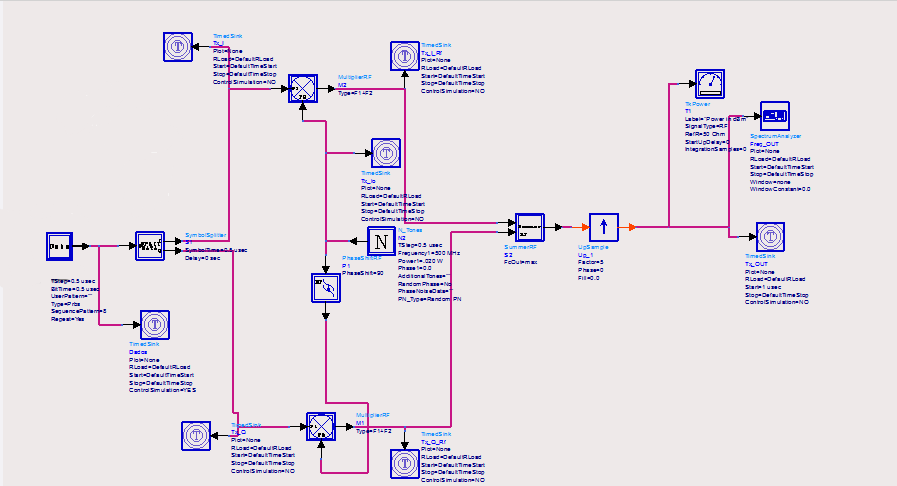
\includegraphics[width=.7\linewidth]{./primeiro_exp/1.png}
\caption{Diagrama de Blocos Referente ao Primeiro Experimento}
\end{figure}


\section{Resultados}

Obtivemos os resultados esperados na simulação, a saída do somador RF é uma boa representação dos dados gerados na entrada do modulador, as vias I e Q são de fato perpendiculares entre si. A constelação QPSK é basicamente a esperada, como explicado na legenda da figura.


\begin{figure}
\centering
\begin{minipage}{.48\textwidth}
  \centering
  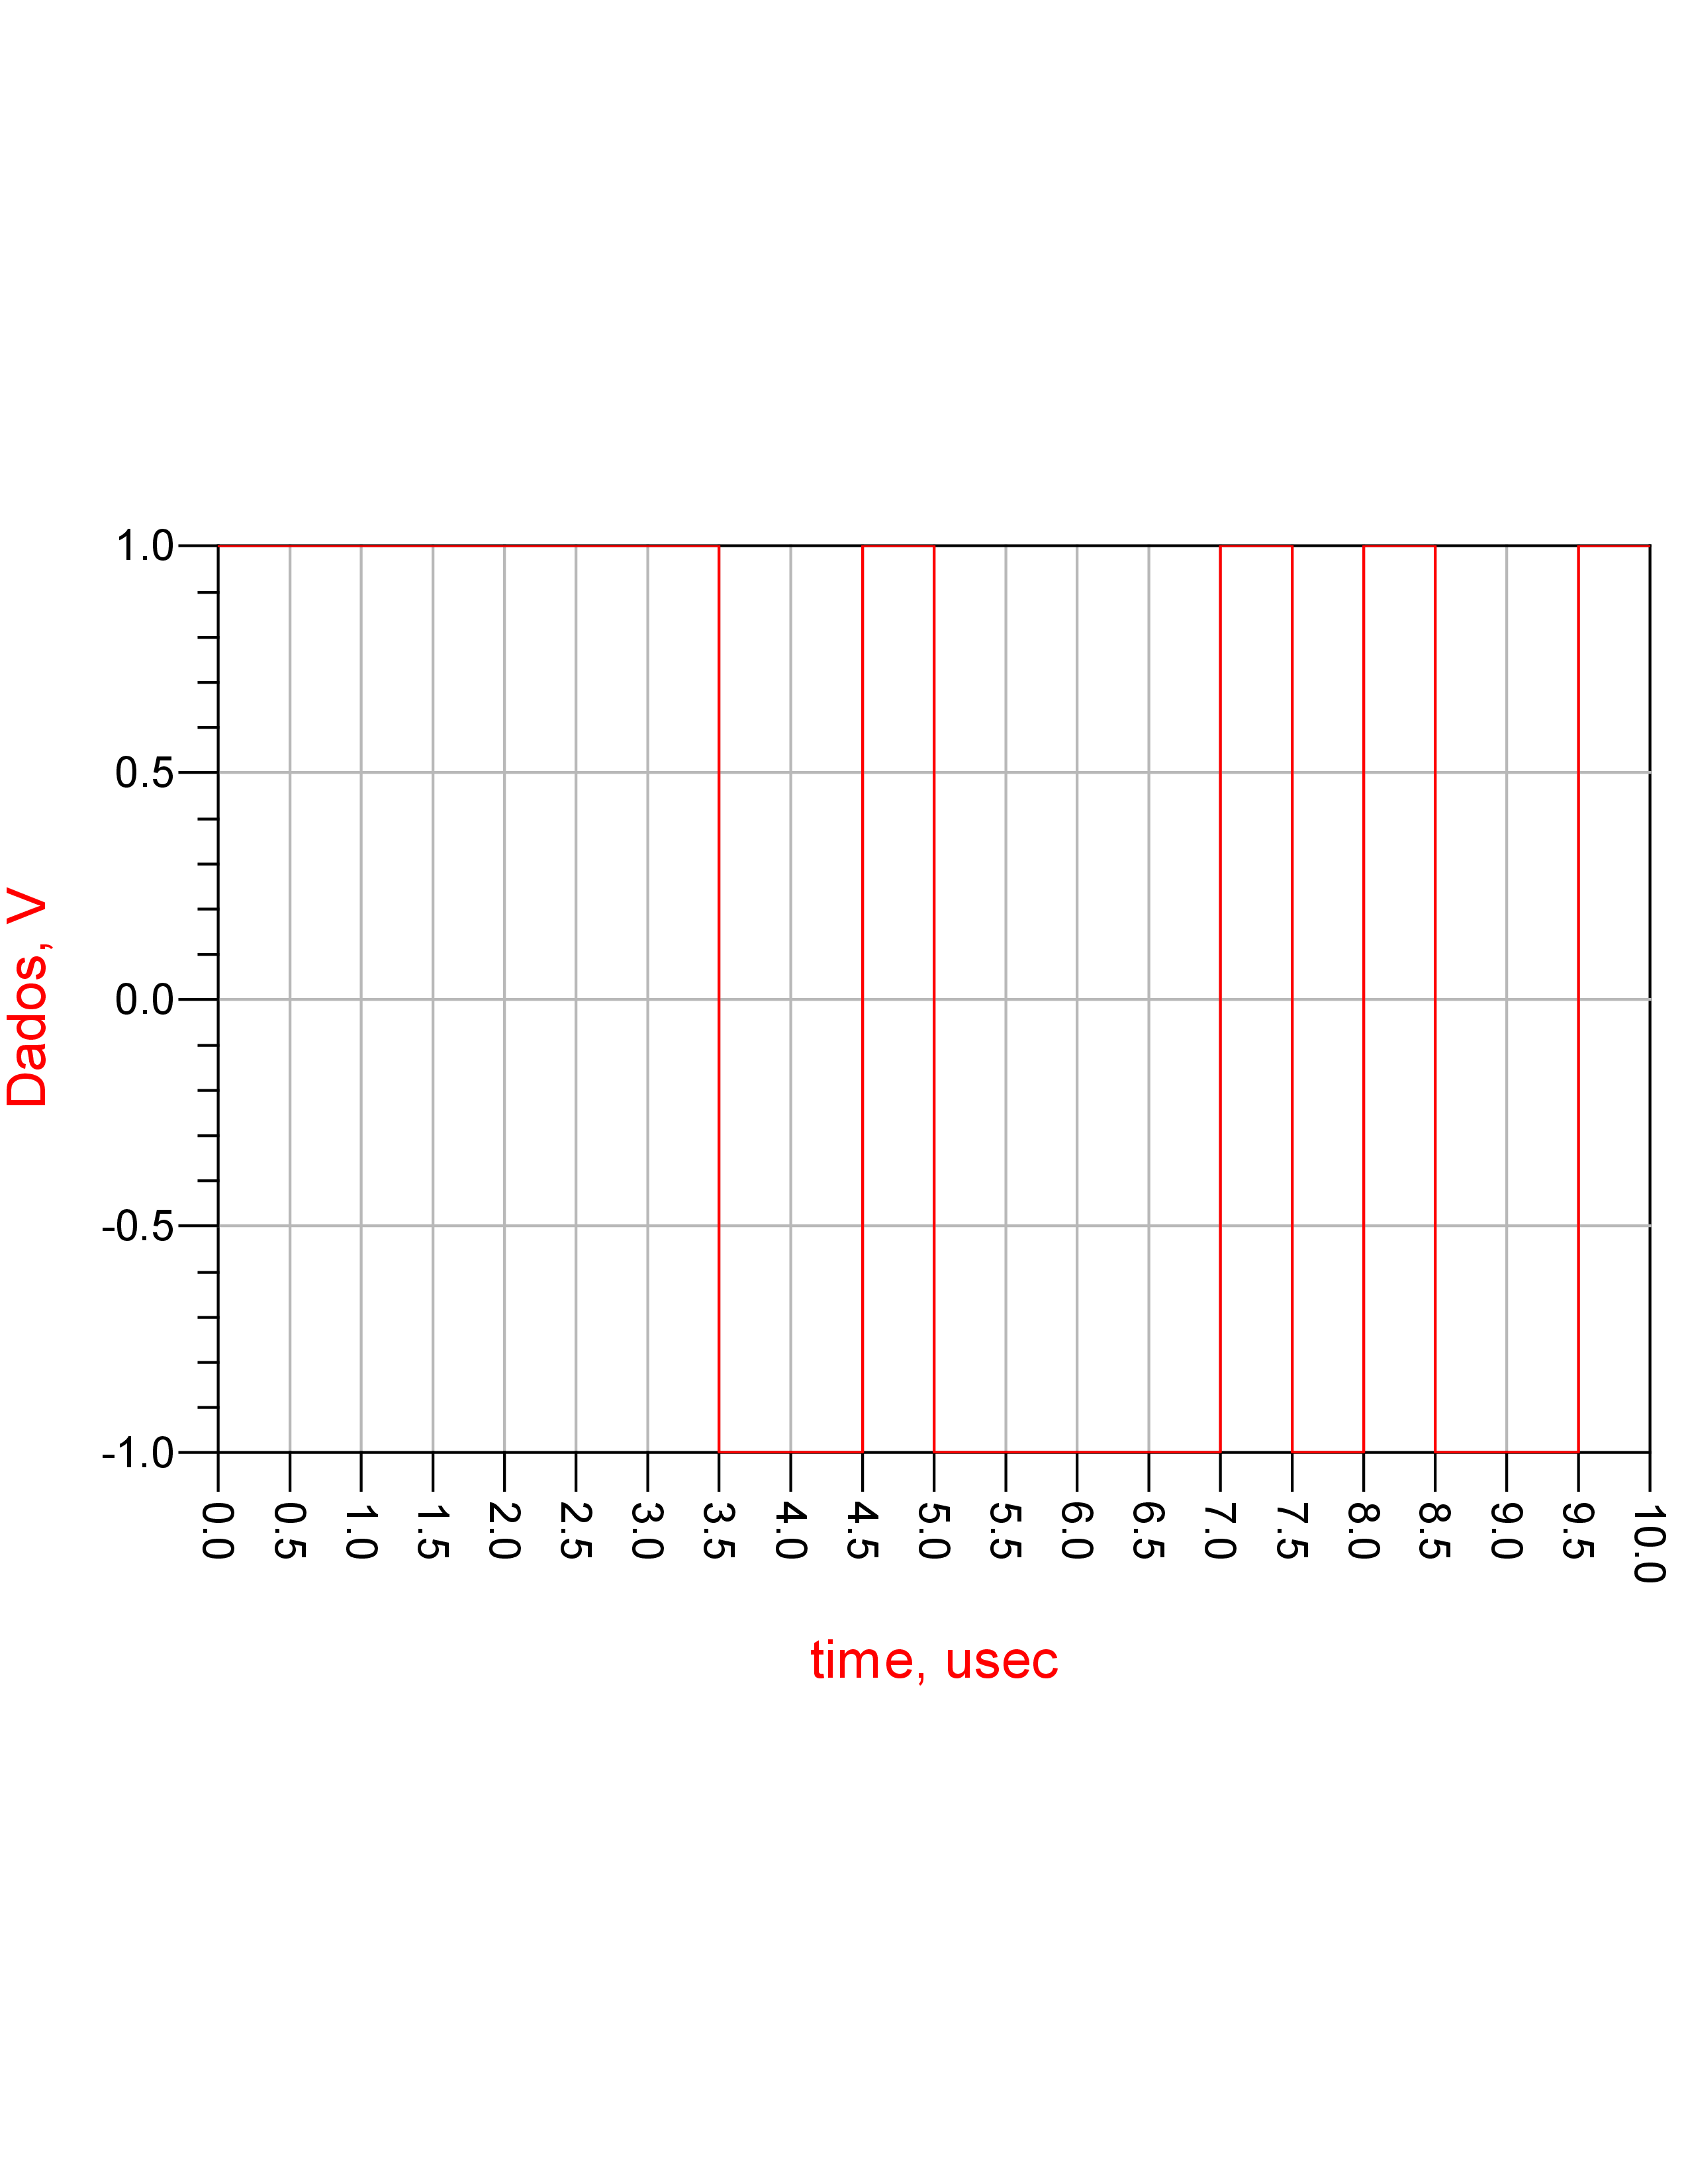
\includegraphics[width=\linewidth]{./primeiro_exp/img3.png}
  \captionof{figure}{Dados Gerados}
  \label{fig:test32}
\end{minipage}%
  \hfill
\begin{minipage}{.48\textwidth}
  \centering
  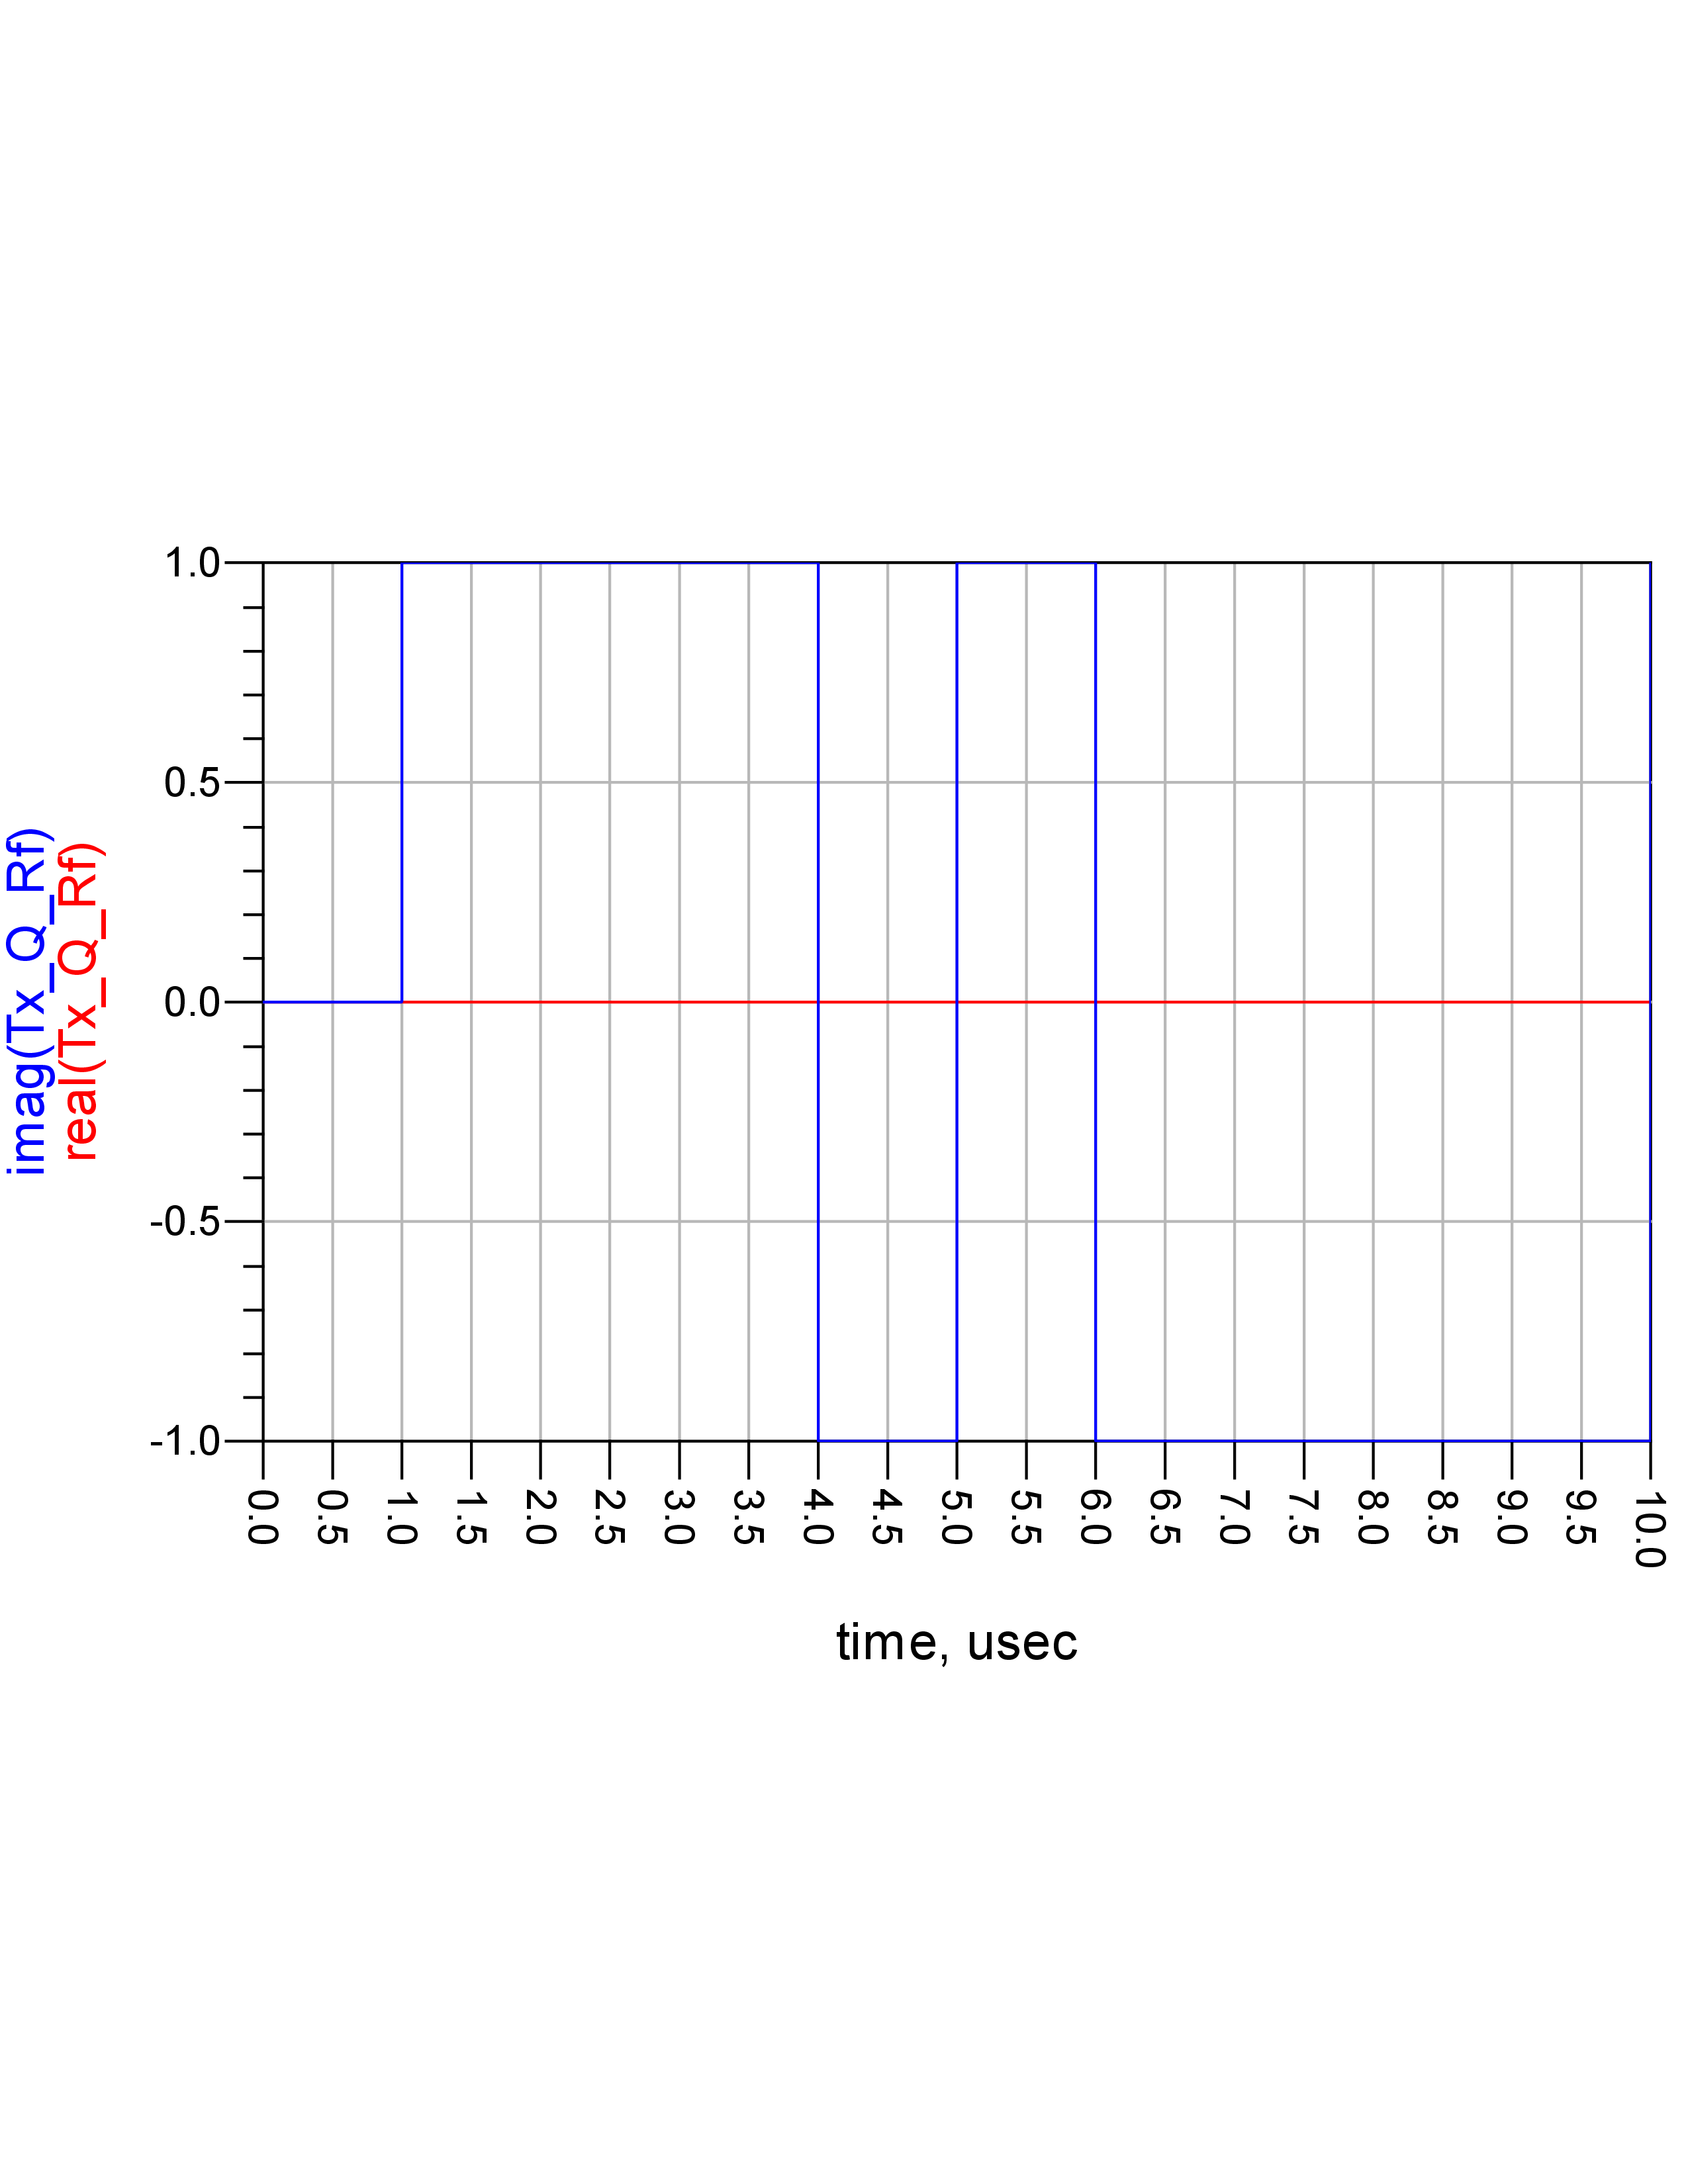
\includegraphics[width=\linewidth]{./primeiro_exp/img5.png}
  \captionof{figure}{Via Q, Parte Real e Imaginária}
  \label{fig:test43}
\end{minipage}
\end{figure}

\begin{figure}
\centering
\begin{minipage}{.48\textwidth}
  \centering
  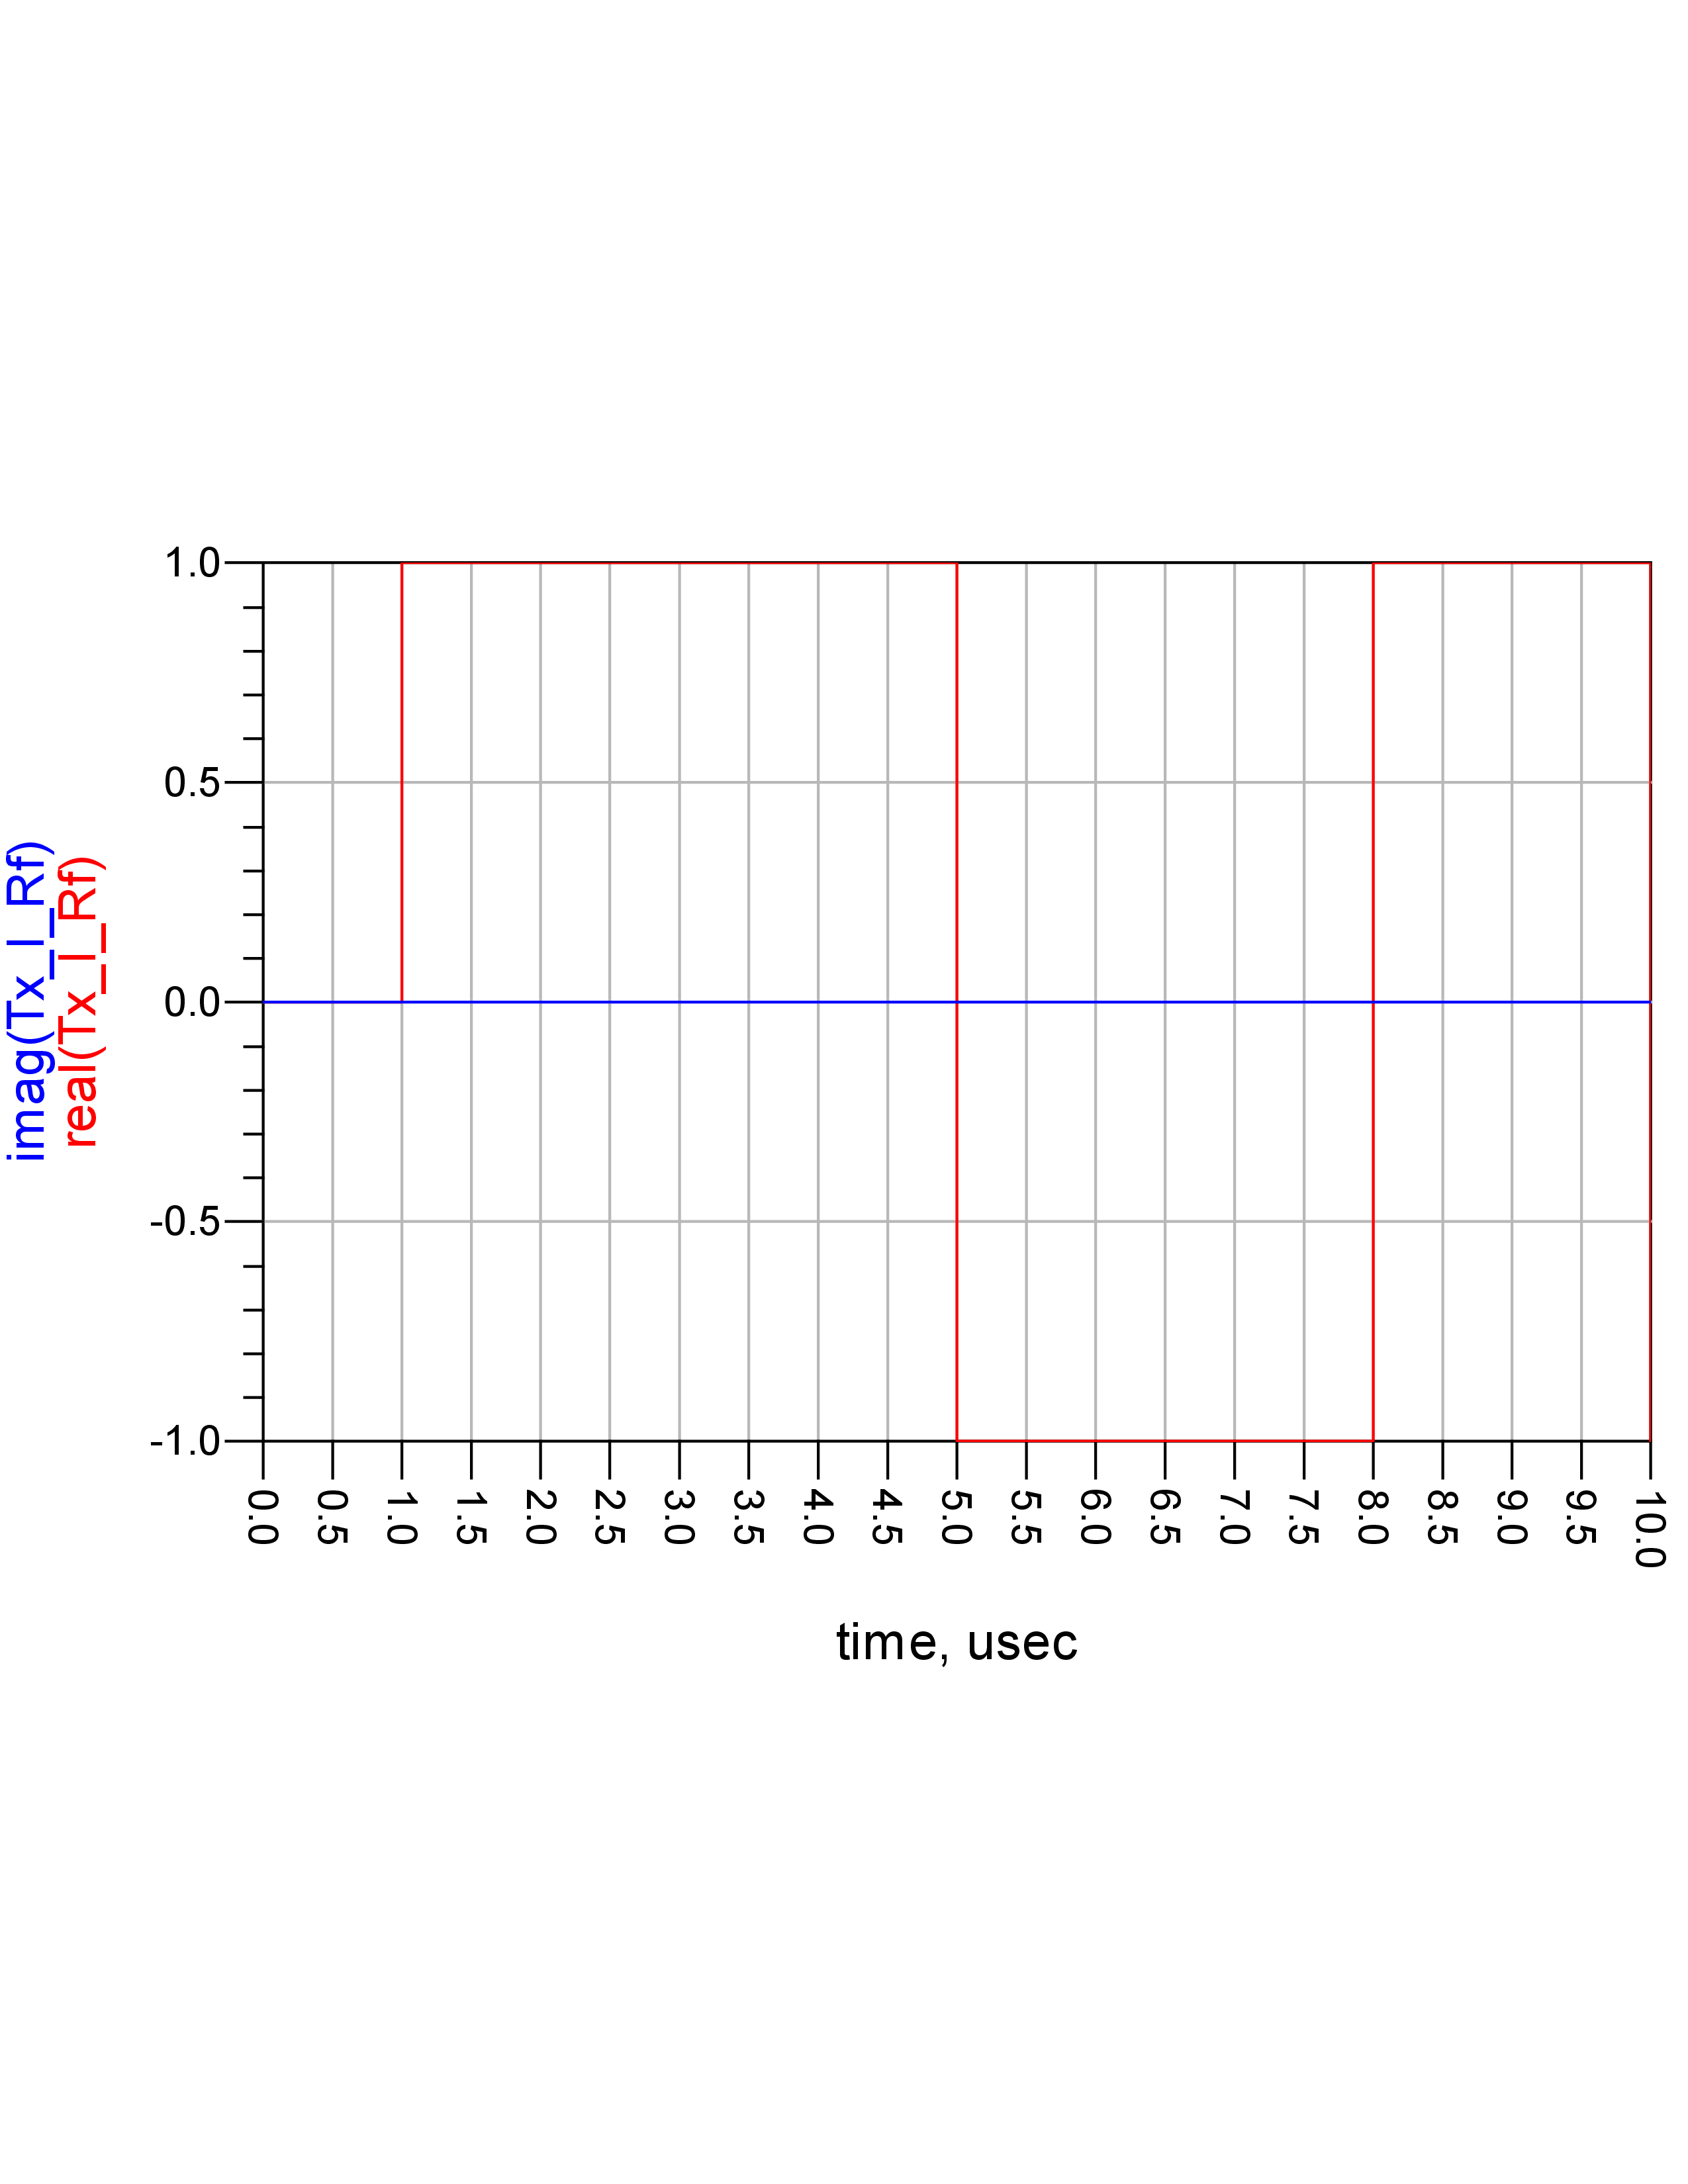
\includegraphics[width=\linewidth]{./primeiro_exp/img4.png}
  \captionof{figure}{Via I, Parte Real e Imaginária}
  \label{fig:test31}
\end{minipage}%
  \hfill
\begin{minipage}{.48\textwidth}
  \centering
  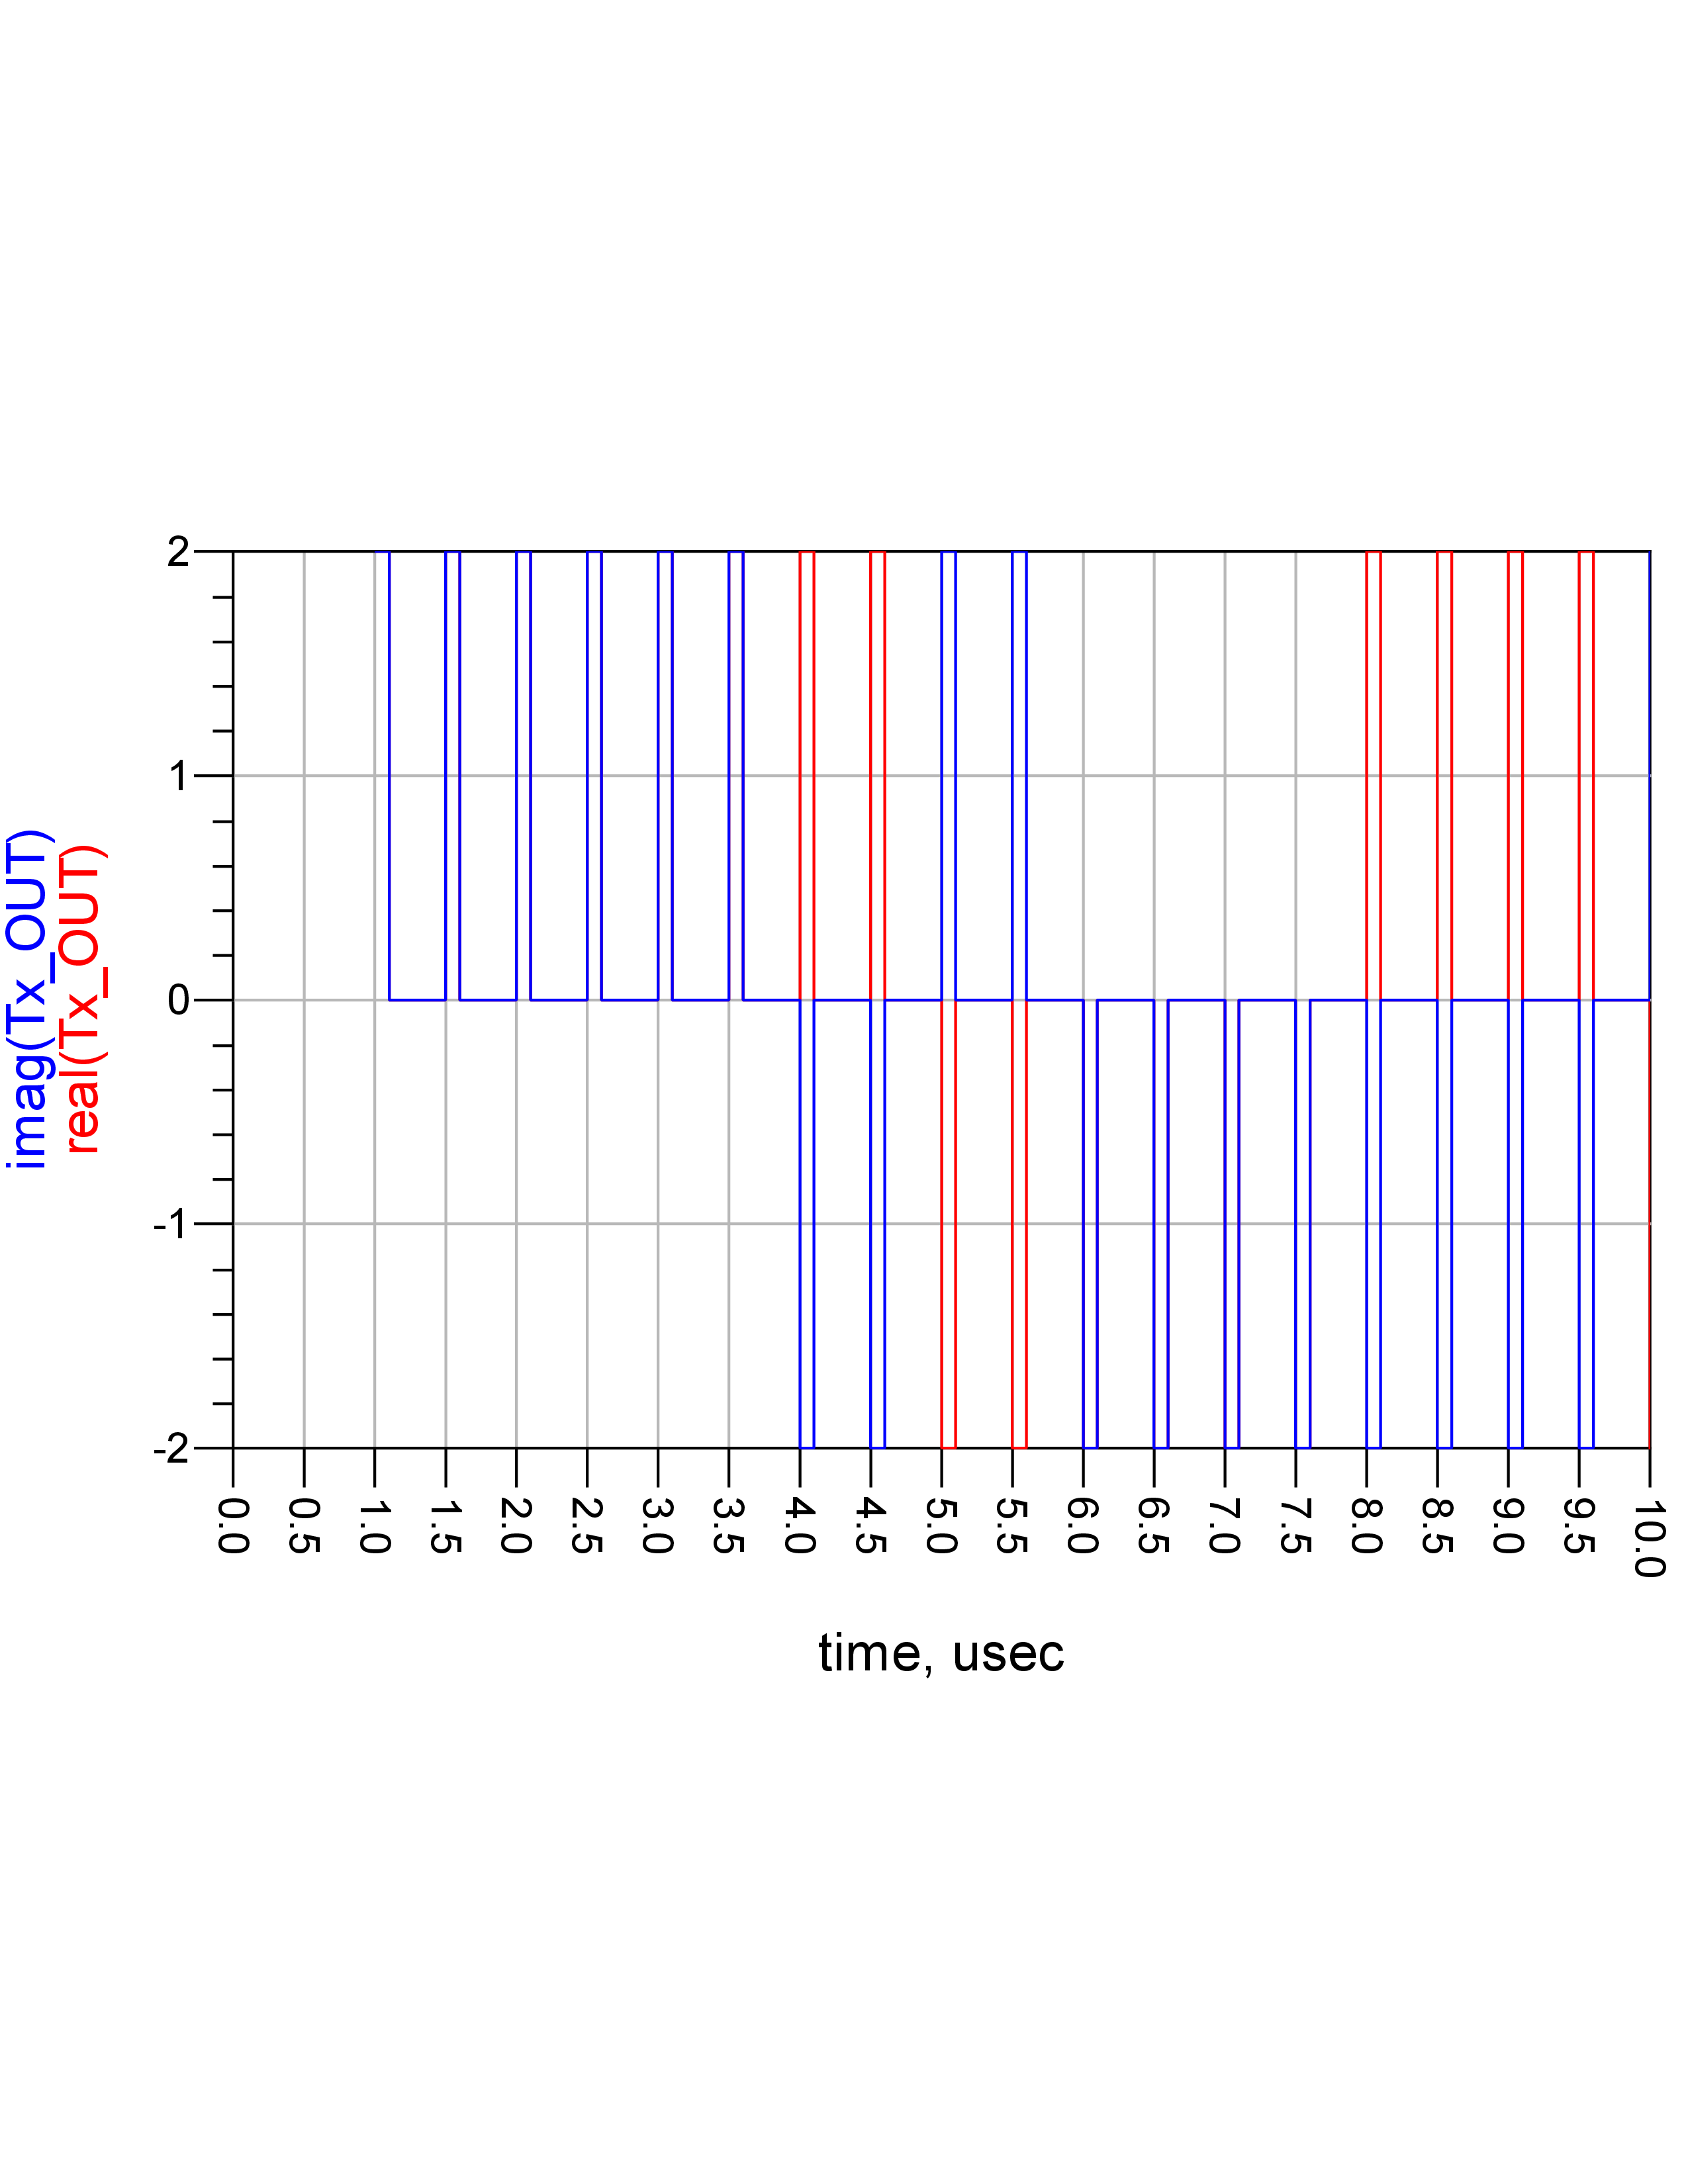
\includegraphics[width=\linewidth]{./primeiro_exp/img6.png}
  \captionof{figure}{Saída do Somador RF, Parte Real e Imaginária}
  \label{fig:test41}
\end{minipage}
\end{figure}
\begin{figure}
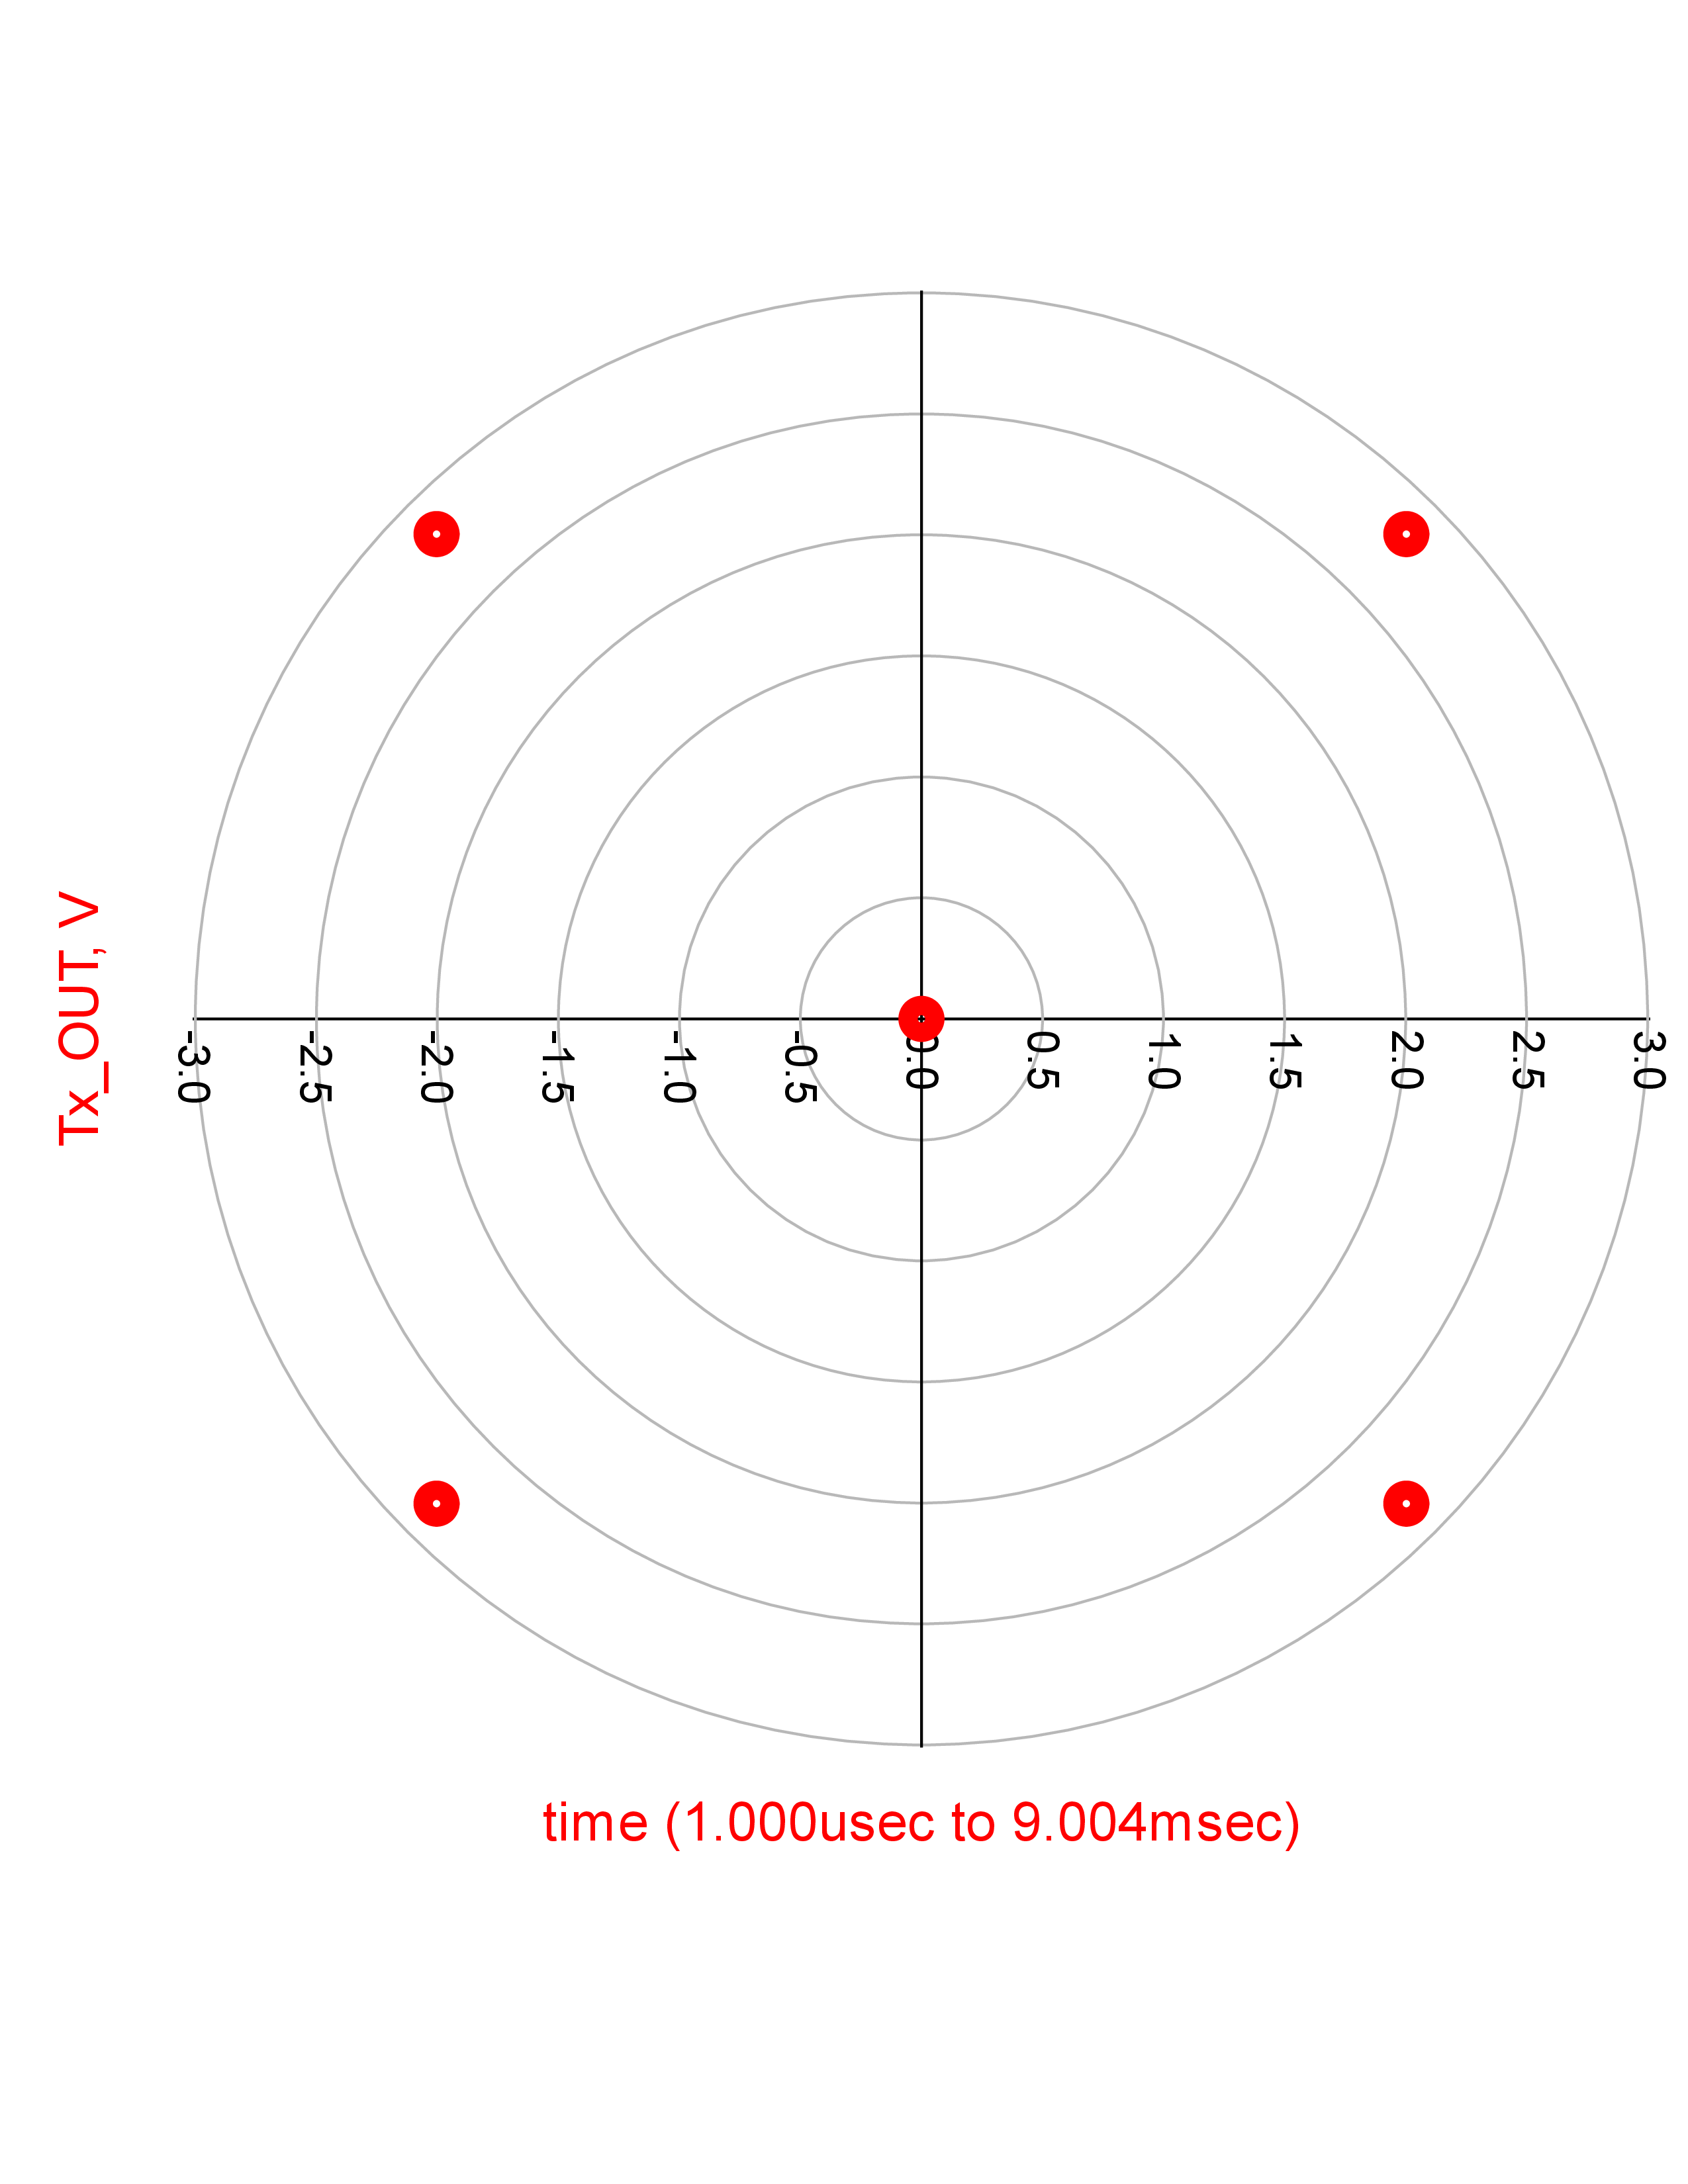
\includegraphics[width=.4\linewidth]{./primeiro_exp/img7.png}
\caption{Constelação QPSK, o ponto no centro da constelação aparece por problemas de casamento de impedância, os 4 pontos deslocados entre si de $90^o$ correspondem aos dados transmitidos, com os pontos no primeiro e terceiro quadrante correspondendo à uma via, e os pontos no segundo e quarto à outra}
\end{figure}

